\chapter{Implementierung des Frameworks}
\label{cap:framework}
In diesem Kapitel werden die technischen Grundlagen sowie das Vorgehen zur Implementierung des Frameworks beschrieben.

\section{Architektur des Frameworks}
\label{sec:architektur_frameowork}
\subsection{Zielsetzung und architektonische Anforderungen}
Der Stand der Technik aktueller Simulationsplattformen für Roboter zeigt, dass
virtuelle Steuerungen und damit zusammenhängende Simulationsplattformen
herstellerspezifisch entwickelt und mit Ausnahme von ROS keine einheitliche
Schnittstelle zur Kommunikation mit externen Plattformen oder Physik-Engines
bieten. Somit muss für jeden Robotertyp ein designierter Konnektor genutzt
werden, um diesen mit einer externen, herstellerunabhängigen Simulationplattform
zu verbinden. Um eine herstellerunabhängige und erweiterbare Plattform zu
entwickeln, sollte also eine gemeinsame Schnittstelle implementiert werden.\\

\noindent
Zusammenfassend verfolgt die Architektur des Frameworks drei zentrale Ziele:
\begin{enumerate}
	\item \textbf{Vendor-Agnostik}: Abstraktion verschiedener Roboterhersteller durch einheitliche Interface-basierte Architektur ohne herstellerspezifische Abhängigkeiten im Kern-Framework

	\item \textbf{Modulare Erweiterbarkeit}: Plugin-System für Safety Monitoring Module und Kommunikationsprotokolle ohne Änderungen der bestehenden Architektur

	\item \textbf{Echtzeitfähige Kommunikation}: Latenzarme Datenübertragung für Motion Control und ereignisbasierte Sicherheitsüberwachung
\end{enumerate}

\subsection{Unity3D als Simulationsplattform}

Die Wahl von Unity3D als zugrundeliegende Simulationsplattform basiert auf
mehreren technischen und praktischen Erwägungen. Während es bereits mehrere
kommerzielle Programme für die Gestaltung und Simulation von Robotern in
virtuellen Umgebungen gibt, sind diese nur selten mit anderen CAD-Systemen und
Robotern kompatibel, unterstützen nicht alle Roboterbibliotheken oder werden
nur plattformabhängig angeboten (vgl. \vglcite[247]{andaluz2016}). Unity3D
hingegen ist mit den meisten CAD-Systemen kompatibel und bietet eine
plattformübergreifende Lösung.\\

\noindent
Unity3D bietet eine ausgereifte 3D-Rendering-Pipeline mit integrierter
Physik-Engine, welche zur Simulation von Gegenständen mit realitätsnahem
Verhalten sowie komplexen Arbeitsräumen geeignet ist \vglcites{\cite@single{Unity2025SystemRequirements};\cite@single{Unity2025PhysicsOverview}}.
Die Engine wurde bereits erfolgreich in der wissenschaftlichen Forschung
eingesetzt und bietet Module und Plugins für spezifische Anwendungsfälle im
Simulationsbereich. Unity3D ermöglicht es auch Nicht-Programmierern,
leistungsstarke Animations- und Interaktionsdesign-Tools zu nutzen, um Roboter
visuell zu programmieren und zu animieren vgl. \vglcite[431]{bartneck2015}.\\

\noindent
Technisch ermöglicht Unity3D durch seine Scripting-Runtime (basierend auf
Mono/.NET Framework) die Verwendung moderner C\#-Sprachfeatures für
nebenläufige Prozesse und asynchroner Programmierung
\vglcite[45-52]{unity_async_2023}, was es ermöglicht, Visualisierung,
Datenakquise und Überwachung zu trennen. Die .NET-basierte Architektur
unterstützt dabei sowohl Task-basierte asynchrone Operationen als auch
Coroutines für zeitgesteuerte Prozesse
\vglcite[123-135]{unity_coroutines_2023}, welche die notwendige periodische
Ausführung von Prozessen auf verschiedenen Ebenen des Frameworks stark
vereinfacht.\\

\noindent
in weiterer Vorteil für die Robotik-Simulation liegt in der
Verfügbarkeit visueller Programmiertools und der integrierten
Entwicklungsumgebung. Die Plattform bietet umfangreiche Debugging- und
Profiling-Werkzeuge (Unity Profiler, Frame Debugger), die während der
Entwicklung und zur Laufzeit genutzt werden können
\vglcite[S.~67-89]{unity_profiler_2023}. Diese Werkzeuge ermöglichen die
Analyse von Performance-Engpässen bei der Verarbeitung von Roboterdaten und die
Optimierung der Sicherheitsmonitor-Updates.

Darüber hinaus lassen sich während der Laufzeit sowohl die Szene (hier: die
Roboterzelle) als auch Komponenten-Parameter in Echtzeit bearbeiten und
einsehen \vglcite[1236]{haas2022}, was das Debuggen und Testen
beschleunigt.

\subsection{Design Patterns und Prinzipien}

Die Entwicklung eines modularen und erweiterbaren Robotersicherheitssystems
erfordert eine fundierte methodische Herangehensweise, die auf bewährten
Software-Engineering-Prinzipien basiert. Die Auswahl geeigneter Design Patterns
und Architekturprinzipien determiniert maßgeblich die Qualitätsattribute des
Systems wie Wartbarkeit, Testbarkeit und
Erweiterbarkeit.\vglcite[73\psqq]{Bass2012} Im Folgenden werden die für diese
Arbeit gewählten Entwurfsmuster und deren Begründung dargelegt.

Für die Realisierung der systemweiten Kommunikation wird das Observer
Pattern\vglcite[293-303]{Gamma1994} als zentrales Entwurfsmuster gewählt. Diese
Entscheidung basiert auf einer zentralen Überlegung: Zunächst muss gewährleistet sein,
dass alle relevanten Ereignisse an relevante Systemkomponenten weitergegeben
werden. Daher ermöglicht das Muster die dynamische Registrierung
und Deregistrierung von Beobachtern zur Laufzeit\vglcite[127\psq]{Buschmann1996} Drittens
reduziert die lose Kopplung zwischen Publisher und Subscriber die
Systemkomplexität erheblich, da Komponenten ohne Kenntnis voneinander
interagieren können.


Die Vorteile dieser Architekturentscheidung manifestiert sich vornehmlich
darin, dass so Robotertypen ohne Modifikation des Kernsystems integriert
werden. \textsc{Martin2003} spricht hier vom Open-Closed-Prinzip, welches die
Offenheit von Software-Entitäten (Funktionen, Klassen, Module, Komponenten
usw.) zur Extension und die gleichzeitige Geschlossenheit zur Modfikation
beschreibt.\vglcite{Martin2003}

\subsubsection{Adapter Pattern zur Hardware-Abstraktion}
Die Integration heterogener Hardware-Komponenten erfordert eine
Abstraktionsschicht zwischen der Anwendungslogik und den hardware-spezifischen
Schnittstellen. Das Adapter Pattern (vgl. \vglcite{Gamma1994}, S. 139-150) wird
gewählt, um diese Abstraktion zu realisieren. Die Notwendigkeit ergibt sich aus
der Vielfalt der Robotersteuerungen und Visualisierungssysteme, die jeweils
eigene APIs und Datenformate verwenden (vgl. \vglcite{Craig2005}, S. 412-415).

Durch die Adapter-Schicht wird eine einheitliche Schnittstelle zur Verfügung
gestellt, die es ermöglicht, verschiedene Robotersysteme ohne Änderung der
Kernlogik anzubinden. Dies reduziert nicht nur die Komplexität des Systems,
sondern erhöht auch dessen Portabilität und Wiederverwendbarkeit (vgl.
\vglcite{Vlissides1995}, S. 89-91).

\subsubsection{SOLID-Prinzipien als Qualitätsfundament}
Die konsequente Anwendung der SOLID-Prinzipien \vglcite{Martin2003} bildet das methodische Fundament der Systemarchitektur. Das
\textit{Single Responsibility Principle} wird angewendet, um kohäsive Module zu
schaffen, die genau eine Verantwortlichkeit haben. Dies reduziert die Kopplung
und erhöht die Verständlichkeit des Codes \vglcite{Martin2017}. Das \textit{Open-Closed Principle} gewährleistet, dass das System für
Erweiterungen offen, aber für Modifikationen geschlossen ist – eine essenzielle
Eigenschaft für langlebige Industriesysteme.

Das \textit{Dependency Inversion Principle} wird konsequent angewendet, indem
High-Level-Module von Abstraktionen abhängen, nicht von konkreten
Implementierungen. Dies ermöglicht die flexible Konfiguration des Systems zur
Laufzeit und vereinfacht die Integration in verschiedene Produktionsumgebungen
\vglcite[112\psqq]{Fowler2018}

\subsubsection{Event-Driven Architecture für Echtzeitfähigkeit}
Die Entscheidung für eine event-getriebene Architektur basiert auf den
Echtzeitanforderungen industrieller Robotersysteme. Sicherheitskritische
Ereignisse müssen innerhalb definierter Zeitschranken verarbeitet werden, was
durch synchrone Aufrufketten nicht gewährleistet werden kann
\vglcite[97\psqq]{Hohpe2003}. Die event-getriebene Architektur ermöglicht die
asynchrone Verarbeitung von Ereignissen und die Priorisierung kritischer
Sicherheitsereignisse.

Zudem adressiert dieser Ansatz die Herausforderung der Integration verschiedener
Datenquellen – von zyklischen Sensordaten über sporadische Alarme bis zu
kontinuierlichen Videoströmen. Jede Datenquelle kann Events in ihrem eigenen
Takt generieren, ohne andere Systemkomponenten zu blockieren
\vglcite[234\psqq]{Vernon2013}.

\section{Schichtenarchitektur des Frameworks}

Aufbauend auf den oben genannte Prinzipien
teilt sich das Framework in 4 logisch getrennte Module auf:

\begin{enumerate}
	\item \textbf{Kernlogik}, welches den Status des Roboters beinhaltet und
	      verwaltet als zentrale Schnittstelle (Core)\item \textbf{Interfaces},
	      welche die Kommunkationsschnittstellen und -methoden zwischen den Modulen
	      implementiert (Interfaces) \item \textbf{Monitoring}, welches die einzelnen
	      Komponenten des Monitoring-Systems implementiert (Monitors) \item
	      \textbf{Adapters}, welches potenziell Adapter zu veschiedenen physischen oder
	      simulierten Steuerungen von Robotern beinhaltet (Hier ABB gennant)
\end{enumerate}



\begin{figure}[H] \centering
	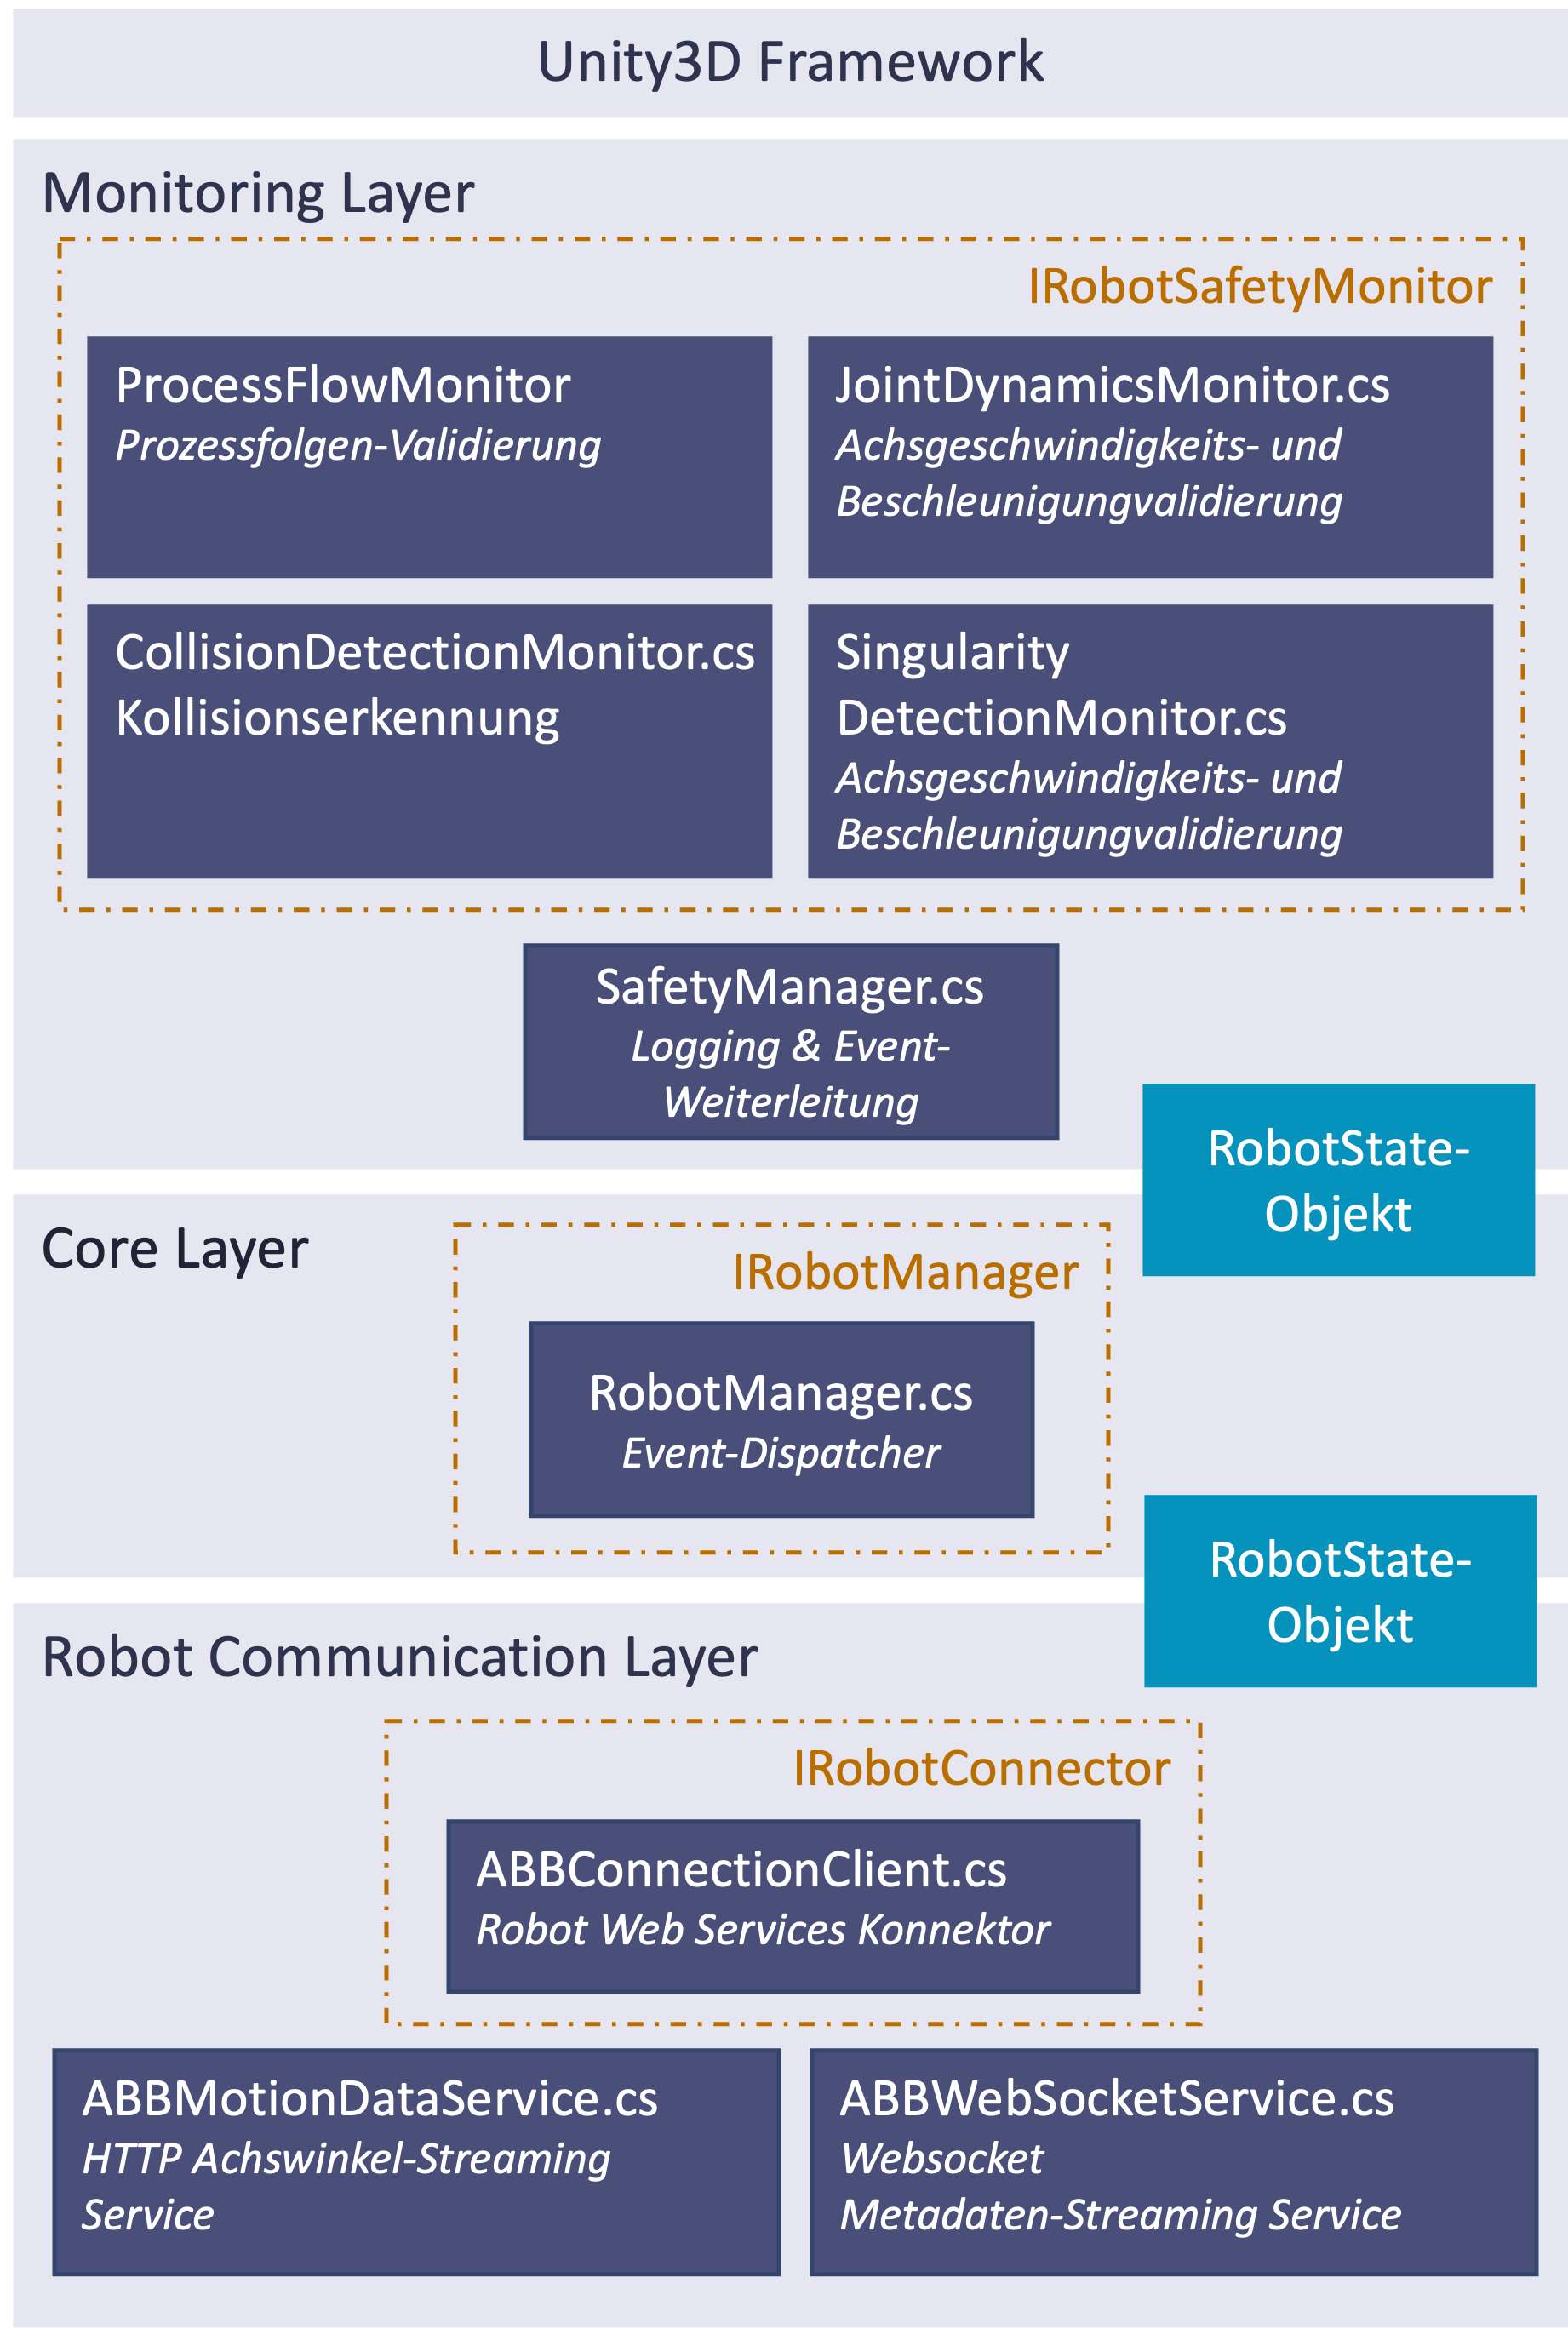
\includegraphics[width=10cm]{Figures/LayerArchitekturFramework.png}
	\caption{Schichtenarchitektur des Frameworks mit den wichtigsten zugehörigen
		Modulen. Module mit grüner Umrandung werden durch eine Interface formalisiert}
	\label{figure:layer}
\end{figure}

Die Trennung der Module ermöglicht eine formalisierte
Schnittstellenkommunikation, dargestellt in Abbildung \ref{figure:layer}.
Jede Schicht hat verschiedene Verantwortlichkeiten und Schnittstellen innerhalb
des Monitoring-Systems. Zentrales Element des Systems stellt der RobotManager
dar. Er dient als Bindeglied zwischen den Monitoring-Komponenten, welche für die
Überwachung des Systems verantworlich sind und der Adapter-Schicht,
verantwortlich für die Kommunikation und das Spiegeln des Roboters aus der
initialen Umgebung (hier RobotStudio) in Unity.

\subsection{Robot Communcation Layer}
Die Robot Communication Layer organisiert die Kommunkation mit der zugrundeliegenden Robotersteuerung und
implentiert eine Interface des Typs IRobotConnector. Als Verbindungsclient
zwischen Unity und externer Schnittstelle des Robotersystems implementiert
dieser eine IRobotConnector Interface, welche als Vorlage für eine Anbindung an
eine Robotersteuerung jedes Typs fungiert und standartisierte Methoden
implementiert:

\begin{figure}[H]
	\inputminted[fontsize=\footnotesize]{csharp}{code-snippets/IRobotConnector.cs}
	\caption{Implementierung der IRobotConnector-Interface als Verbidung zwischen
		RobotState und Roboter-Controller}
\end{figure}
\noindent
Eine Interface lässt sich anhand dieses Beispiels in \textbf{3
	Funktionsbereiche} aufteilen: Events, Attribute und Methoden.\\

\noindent
Die Interface definiert \textbf{Events (Aktionen)} die bei definierten Zustandsänderungen
in der Laufzeit ausgeführt werden. Andere Bestandteile des Framework sind in der
Lage, ein Event zu abonnieren und eine Methode registieren, welche ausgeführt
werden soll, wenn dieses Event auftritt. Ist dies der Fall, wird das
entsprechende Modul über die Änderung benachrichtigt und bekommt gegebenfalls
neue Daten zur Verfügung gestellt. Diese event-getriebene Kommunikation sorgt
dafür, dass einerseits alle Komponenten proaktiv auf den neusten Stand der Daten gebracht
und gehalten werden, andererseits aber keine ressourcenblockierenden Prozesse
ausgeführt werden müssen, um gegebenfalls Statusänderungen abzufragen.\\

\noindent
Weiterführend definiert die Interface IRobotConnector \textbf{Attribute}, welche den
aktuellen Verbindungsstatus (verbunden = \texttt{true}, getrennt = \texttt{false}) speichern sowie das
State-Objekt des Roboters. Definiert durch die schreibgeschützten, automatisch
implementierte Eigenschaft mit einem Getter \textit{\{ get; \}} können Attribute
auch von ausserhalb des RobotConnectors abgefragt werden, jedoch nicht
überschrieben.\\

\noindent
Zuletzt gibt die Interface die Methoden \textit{\textbf{Connect}} und \textit{\textbf{Disconnect}}
vor, welche hier die wichtigsten Methoden zum Verbinden und
Trennen von der jeweiligen Robotersteuerung darstellen.

Als initiale Komponente wird eine Verbindung zum
Controller eines Roboters benötigt, um den Roboter in Unity emulieren zu können
und Daten zu verarbeiten. Dazu wird hier mittels eines HTTP-Clients zur
Schnittstelle des RobotStudioSDKs über die API RobotWebServices (RWS) eine
Verbindung aufgebaut. Die Verbindung zu RobotWebServices ensteht durch einen
HTTP-Client und der Authentifizierung mit in RobotStudio festgelegten
Zugangsdaten. Anschliessend kann über einen erhaltenen Cookie die Verbindung
aufrecherhalten werden und aktuelle Daten über den Roboter sowohl abgefragt,
also auch der Roboter selbst gesteuert werden.\vglcite{robotwebservices2025}

Die RWS-Schnittstelle bietet einerseits die Möglichkeiten,
aktuellen Achswinkel und TCP-Werte (Tool Center Point) abzurufen, als auch
weitere Metadaten, wie das aktuell laufende Programm, den aktuellen Motorstatus
oder auch die Codezeile, welche aktuell vom Programmzeiger ausgeführt wird.
Weiterführend bietet RWS die Möglichkeit, die aktuelle digitale und analoge
Signale abzurufen, was nötig ist, um den Greifer steuern zu können.

Bei den oben genannten Daten mit Ausnahme der Achswinkel handelt es sich um
Paramenter, welche sich im Laufe eines Programmablaufs vergleichsweise selten
verändern. Daher wird hier auf den Websockets-Endpunkt von RWS zugegriffen, um
innerhalb einer Duplex-Kommunikation sich verändernende Signale oder auch
Programmstati zu empfangen. Dazu wird mithilfe des HTTP-Clients eine Anfrage zur
Subscription auf verschiedene Parameter (bspw. den ProgrammPointer) gestellt,
und anschliessend eine Websockets-Session aufgebaut. Die Achswinkel werden
zeitgleich über eine asynchron endlosen Task in einer in Unity definierbaren
Frequenz abgefragt.

Der Client implementiert dabei die Interface IRobotConnector und gibt ein
RobotState-Objekt mit den empfangenen Daten an den RobotManager weiter, welcher hier
als zentraler Koordinator des aktuellen RobotState fungiert.

\noindent
\paragraph{Event-Driven Architecture}
as System nutzt ein durchgängiges Event-System für lose Kopplung:
\begin{itemize}
	\item \texttt{OnRobotStateUpdated}: Zustandsänderungen
	\item \texttt{OnConnectionStateChanged}: Verbindungsstatus
	\item \texttt{OnSafetyEventDetected}: Sicherheitsereignisse
	\item \texttt{OnMotorStateChanged}: Motorstatusänderungen
\end{itemize}

\paragraph{SafetyEvent und RobotStateSnapshot}
Als für die Auswertung der Simulationsergebnisse relevantes Teil des Frameworks
wird eine SaftetyEvent-Objekt implementiert. Jedes Mal, wenn ein Ereignis,
welches mit der tatsächlichen Simluation eines Roboterpgrogramms zusammenhängt,
auftritt, wird ein SafetyEvent instanziert. Dieses wird initial von der
jeweiligen überwachenden Komponente (einem SafetyMonitor) instanziert und mit
dem aktuellsten RobotState als unveränderliches Objekt (RobotStateSnapshot) befüllt.
Weiterführend erhält es vom jeweiligen SafetyMonitor variierende
Kontextinformationen, die später für die Auswertung des Ereignisses verwendet
werden. Zusammenfassend bestehn ein SafetyEvent aus folgenden Komponenten:
\begin{itemize}
	\item \textbf{SafetyEvent}: Unveränderliches Value Object für Sicherheitsereignisse
	\item \textbf{RobotStateSnapshot}: Immutable Zustandserfassung zum Ereigniszeitpunkt
	\item \textbf{Ereignistypen}: Info, Warning, Critical mit konfigurierbaren Schwellwerten
	\item \textbf{Kontextdaten}: Vollständige Roboterzustandserfassung für Forensik
\end{itemize}
\noindent

\dirtree{%
	.1 RobotSystem/.
	.2 Core/.
	.3 RobotManager.cs.
	.3 RobotState.cs.
	.3 RobotSafetyManager.cs.
	.3 SafetyEvent.cs.
	.3 RobotStateSnapshot.cs.
	.3 Part.cs.
	.3 Station.cs.
	.3 RapidTargetGenerator.cs.
	.2 Interfaces/.
	.3 IRobotConnector.cs.
	.3 IRobotDataParser.cs.
	.3 IRobotSafetyMonitor.cs.
	.3 IRobotVisualization.cs.
	.2 ABB/.
	.3 RWS/.
	.4 ABBRWSConnectionClient.cs.
	.4 ABBRWSDataParser.cs.
	.4 ABBMotionDataService.cs.
	.3 ABBFlangeAdapter.cs.
	.2 Monitors/.
	.3 CollisionDetectionMonitor.cs.
	.3 JointDynamicsMonitor.cs.
	.3 ProcessFlowMonitor.cs.
	.3 SingularityDetectionMonitor.cs.
}

s

\subsection{Zielsetzung und architektonische Anforderungen}

Daher verfolgt das Framework verfolgt drei \textbf{zentrale architektonische
	Ziele}:

\begin{enumerate}
	\item \textbf{Vendor-Agnostik}: Abstraktion verschiedener Roboterhersteller durch einheitliche Interface-basierte Architektur ohne herstellerspezifische Abhängigkeiten im Kern-Framework

	\item \textbf{Modulare Erweiterbarkeit}: Plugin-System für Safety Monitoring Module und Kommunikationsprotokolle ohne Änderungen der bestehenden Architektur

	\item \textbf{Echtzeitfähige Kommunikation}: Latenzarme Datenübertragung für Motion Control und ereignisbasierte Sicherheitsüberwachung
\end{enumerate}

\subsection{Unity3D als Simulationsplattform}

\subsubsection{Auswahl und Vorteile gegenüber Alternativen}

Die Wahl von Unity3D als zugrundeliegende Simulationsplattform basiert auf
mehreren technischen und praktischen Erwägungen. Während es bereits mehrere
kommerzielle Programme für die Gestaltung und Simulation von Robotern in
virtuellen Umgebungen gibt, sind diese nur selten mit anderen CAD-Systemen und
Robotern kompatibel, unterstützen nicht alle Roboterbibliotheken oder werden
nur plattformabhängig angeboten (vgl. \vglcite[247]{andaluz2016}). Unity3D
hingegen ist mit den meisten CAD-Systemen kompatibel und bietet eine
plattformübergreifende Lösung.

\subsubsection{3D-Rendering und Physik-Simulation}

Unity3D bietet eine ausgereifte 3D-Rendering-Pipeline mit integrierter
Physik-Engine, welche zur Simulation von Gegenständen mit realitätsnahem
Verhalten sowie komplexen Arbeitsräumen geeignet ist (vgl.
\vglcite{Unity2025SystemRequirements}, \vglcite{Unity2025PhysicsOverview}). Die
Engine wurde bereits erfolgreich in der wissenschaftlichen Forschung eingesetzt
und bietet Module und Plugins für spezifische Anwendungsfälle im
Simulationsbereich. Unity3D ermöglicht es auch Nicht-Programmierern,
leistungsstarke Animations- und Interaktionsdesign-Tools zu nutzen, um Roboter
visuell zu programmieren und zu animieren (vgl. \vglcite[431]{bartneck2015}).

\subsubsection{Technische Architektur und Programmierung}

Technisch ermöglicht Unity3D durch seine Scripting-Runtime (basierend auf
Mono/.NET Framework) die Verwendung moderner C\#-Sprachfeatures für
nebenläufige Prozesse und asynchroner Programmierung
\vglcite[S.~45-52]{unity_async_2023}, was es ermöglicht, Visualisierung,
Datenakquise und Überwachung zu trennen. Die .NET-basierte Architektur
unterstützt dabei sowohl Task-basierte asynchrone Operationen als auch
Coroutines für zeitgesteuerte Prozesse
\vglcite[S.~123-135]{unity_coroutines_2023}, welche die notwendige periodische
Ausführung von Prozessen auf verschiedenen Ebenen des Frameworks stark
vereinfacht.

Die Unity-Engine unterstützt nativ Multithreading durch das Job System
\vglcite[S.~201-218]{unity_jobsystem_2023}, was für die parallele Verarbeitung
von Sensordaten, Kollisionserkennung und Bewegungsplanung entscheidend ist.

\subsubsection{Entwicklungsumgebung und Debugging-Tools}

Ein weiterer entscheidender Vorteil für die Robotik-Simulation liegt in der
Verfügbarkeit visueller Programmiertools und der integrierten
Entwicklungsumgebung. Die Plattform bietet umfangreiche Debugging- und
Profiling-Werkzeuge (Unity Profiler, Frame Debugger), die während der
Entwicklung und zur Laufzeit genutzt werden können
\vglcite[S.~67-89]{unity_profiler_2023}. Diese Werkzeuge ermöglichen die
Analyse von Performance-Engpässen bei der Verarbeitung von Roboterdaten und die
Optimierung der Sicherheitsmonitor-Updates.

Darüber hinaus lassen sich während der Laufzeit sowohl die Szene (hier: die
Roboterzelle) als auch Komponenten-Parameter in Echtzeit bearbeiten und
einsehen \vglcite[S.~1236]{haas_realtime_2022}, was das Debuggen und Testen
beschleunigt.

\subsubsection{Benutzerfreundlichkeit und industrielle Anwendung}

Besonders relevant für industrielle Robotik-Anwendungen ist die Möglichkeit,
Custom Editor Scripts zu entwickeln (vgl.
\vglcite[S.~156-172]{unity_editors_2023}), die eine benutzerfreundliche und
niederschwellige Konfiguration verschiedener Parameter ermöglichen. Zusätzlich
ermöglichen Gizmos und Scene View die visuelle Darstellung von Kollisionszonen,
Singularitätspunkten und Prozessabläufen während der Entwicklung (vgl.
\vglcite[S.~234-245]{unity_gizmos_2023}).

\subsection{Design Patterns und Prinzipien}

Die Entwicklung eines modularen und erweiterbaren Robotersicherheitssystems
erfordert eine fundierte methodische Herangehensweise, die auf bewährten
Software-Engineering-Prinzipien basiert. Die Auswahl geeigneter Design Patterns
und Architekturprinzipien determiniert maßgeblich die Qualitätsattribute des
Systems wie Wartbarkeit, Testbarkeit und Erweiterbarkeit (vgl.
\vglcite{Bass2012}, S. 73-75). Im Folgenden werden die für diese Arbeit
gewählten Entwurfsmuster und deren Begründung dargelegt.

\subsubsection{Observer Pattern als Kommunikationsparadigma}
Für die Realisierung der systemweiten Kommunikation wird das Observer Pattern
(vgl. \vglcite{Gamma1994}, S. 293-303) als zentrales Entwurfsmuster gewählt.
Diese Entscheidung basiert auf drei wesentlichen Anforderungen industrieller
Robotersysteme: Erstens müssen Sicherheitsereignisse ohne Verzögerung an alle
relevanten Systemkomponenten propagiert werden, was durch die inhärente
Entkopplung des Observer Patterns gewährleistet wird. Zweitens ermöglicht das
Muster die dynamische Registrierung und Deregistrierung von Beobachtern zur
Laufzeit, was für modulare Sicherheitssysteme unerlässlich ist (vgl.
\vglcite{Buschmann1996}, S. 127-128). Drittens reduziert die lose Kopplung
zwischen Publisher und Subscriber die Systemkomplexität erheblich, da
Komponenten ohne Kenntnis voneinander interagieren können.

Das Observer Pattern adressiert zudem die Herausforderung der
Multi-Threading-Umgebung in Unity3D, indem Events asynchron verarbeitet werden
können, ohne den Hauptthread zu blockieren (vgl. \vglcite{Nystrom2014}, S.
156-159). Dies ist besonders kritisch für die Echtzeitverarbeitung von
Sensordaten und die gleichzeitige Visualisierung.

\subsubsection{Strategy Pattern für algorithmische Flexibilität}
Die Wahl des Strategy Patterns (vgl. \vglcite{Gamma1994}, S. 315-323) für die
Implementierung von Sicherheitsmonitoren und Datenparser begründet sich durch
die Heterogenität industrieller Robotersysteme. Verschiedene Roboterhersteller
verwenden proprietäre Kommunikationsprotokolle und Datenformate, was eine
flexible Austauschbarkeit von Parsing-Algorithmen erfordert (vgl.
\vglcite{Siciliano2016}, S. 891-893). Das Strategy Pattern kapselt diese
Algorithmen in separaten Klassen und macht sie über eine gemeinsame
Schnittstelle austauschbar.

Die Vorteile dieser Architekturentscheidung manifestiert sich vornehmlich
darin, dass so Robotertypen ohne Modifikation des Kernsystems integriert
werden. \textsc{Martin2003} spricht hier vom Open-Closed-Prinzip, welches die
Offenheit von Software-Entitäten (Funktionen, Klassen, Module, Komponenten
usw.) zur Extension und die gleichzeitige Geschlossenheit zur Modfikation
beschreibt.\vglcite{Martin2003}

\subsubsection{Adapter Pattern zur Hardware-Abstraktion}
Die Integration heterogener Hardware-Komponenten erfordert eine
Abstraktionsschicht zwischen der Anwendungslogik und den hardware-spezifischen
Schnittstellen. Das Adapter Pattern (vgl. \vglcite{Gamma1994}, S. 139-150) wird
gewählt, um diese Abstraktion zu realisieren. Die Notwendigkeit ergibt sich aus
der Vielfalt der Robotersteuerungen und Visualisierungssysteme, die jeweils
eigene APIs und Datenformate verwenden (vgl. \vglcite{Craig2005}, S. 412-415).

Durch die Adapter-Schicht wird eine einheitliche Schnittstelle zur Verfügung
gestellt, die es ermöglicht, verschiedene Robotersysteme ohne Änderung der
Kernlogik anzubinden. Dies reduziert nicht nur die Komplexität des Systems,
sondern erhöht auch dessen Portabilität und Wiederverwendbarkeit (vgl.
\vglcite{Vlissides1995}, S. 89-91).

\subsubsection{SOLID-Prinzipien als Qualitätsfundament}
Die konsequente Anwendung der SOLID-Prinzipien (vgl. \vglcite{Martin2003}, S.
95-135) bildet das methodische Fundament der Systemarchitektur. Das
\textit{Single Responsibility Principle} wird angewendet, um kohäsive Module zu
schaffen, die genau eine Verantwortlichkeit haben. Dies reduziert die Kopplung
und erhöht die Verständlichkeit des Codes (vgl. \vglcite{Martin2017}, S.
62-64). Das \textit{Open-Closed Principle} gewährleistet, dass das System für
Erweiterungen offen, aber für Modifikationen geschlossen ist – eine essenzielle
Eigenschaft für langlebige Industriesysteme.

Das \textit{Dependency Inversion Principle} wird konsequent angewendet, indem
High-Level-Module von Abstraktionen abhängen, nicht von konkreten
Implementierungen. Dies ermöglicht die flexible Konfiguration des Systems zur
Laufzeit und vereinfacht die Integration in verschiedene Produktionsumgebungen
(vgl. \vglcite{Fowler2018}, S. 112-115).

\subsubsection{Event-Driven Architecture für Echtzeitfähigkeit}
Die Entscheidung für eine event-getriebene Architektur basiert auf den
Echtzeitanforderungen industrieller Robotersysteme. Sicherheitskritische
Ereignisse müssen innerhalb definierter Zeitschranken verarbeitet werden, was
durch synchrone Aufrufketten nicht gewährleistet werden kann (vgl.
\vglcite{Hohpe2003}, S. 97-99). Die event-getriebene Architektur ermöglicht die
asynchrone Verarbeitung von Ereignissen und die Priorisierung kritischer
Sicherheitsereignisse.

Zudem adressiert dieser Ansatz die Herausforderung der Integration
verschiedener Datenquellen – von zyklischen Sensordaten über sporadische Alarme
bis zu kontinuierlichen Videoströmen. Jede Datenquelle kann Events in ihrem
eigenen Takt generieren, ohne andere Systemkomponenten zu blockieren (vgl.
\vglcite{Vernon2013}, S. 234-237).

\subsection{Systemarchitektur und Entwurfsmuster}

\subsubsection{Flange Framework als Visualisierungs- und Konfigurationstool}
Im Rahmen dieses Frameworks wird das Unity-Package
\textit{Flange} genutzt. Implementiert durch GitHub-User \textit{Preliy} und frei
verfügbar im Rahmen einer BSD 3-Clause Lizenz, bietet ein spezialisiertes
Framework für die Robotersteuerung in Unity mit modularer Architektur, die
Gelenksteuerung, Kinematik, Koordinatentransformationen und Echtzeitüberwachung
als separate Komponenten organisiert. Das System unterstützt sowohl direkte
Gelenkmanipulation auf niedriger Ebene als auch kartesische Steuerung auf
höherer Abstraktionsebene, wodurch es für verschiedene Roboteranwendungen
einsetzbar ist.\vglcite{preliyflange2024} Im Kontext dieser Entwicklungsarbeit wird Flange zur
Implementierung und Visualisierung der Denavit-Hartenberg-Parameter und damit
einhergehender Achstransformationen eingesetzt,
da diese Notation als fundamentales Werkzeug der Robotik eine systematische
Beschreibung der Geometrie serieller Robotermechanismen ermöglicht und somit die
Anwendung etablierter algorithmischer Verfahren für kinematische Berechnungen,
Jacobi-Matrizen sowie Bewegungsplanung unterstützt.\vglcite[590]{corke2007}

Flange ermöglicht eine direkte Konfiguration des Roboters über \textit{Frame}
und \textit{JointTransformation} Scripts. Ein Frame definiert dabei die
Denavit-Hartenberg-Parameter für einen Teil der kinematischen Kette, eine
JointTransformation die Paramter des Gelenks, also möglicher maximaler Ausschlag
in positive und negative Achsrotationsrichtung sowie maximale Geschwindigkeit
und Beschleunigung. Diese Funktion werden im Rahmen dieser Implentierung
genutzt, um den zu simulierenden Roboter theoretisch nachvollziehbar im Raum
bewegen zu können.

\subsubsection{Schichtenarchitektur}
Aufbauend auf den oben genannte Prinzipien teilt sich das Framework in 4
logisch getrennte Module auf:
\begin{enumerate}
	\item \textbf{Kernlogik}, welches den Status des Roboters beinhaltet und verwaltet als
	      zentrale Schnittstelle (Core)
	\item \textbf{Interfaces}, welche die Kommunkationsschnittstellen und -methoden
	      zwischen den Modulen implementiert (Interfaces)
	\item \textbf{Monitoring}, welches die einzelnen Komponenten des Monitoring-Systems
	      implementiert (Monitors)
	\item \textbf{Adapters}, welches potenziell Adapter zu veschiedenen physischen oder
	      simulierten Steuerungen von Robotern beinhaltet (Hier ABB gennant)
\end{enumerate}
Beispielhaft wird im Folgenden erläutert, aus welchen Bestandenteilen Interfaces
des Framework bestehen. Da jedes Modul, welches von einer Interface erbt
zwangsweise dessen Komponenten implenentieren muss, lassen sich hierdurch die
grundlegenden Funktionalitäten des Framework abstrahieren.

\subsubsection{Interfaces}
Die Trennung der Module ermöglicht eine formalisierte
Schnittstellenkommunikation, dargestellt in Abbildung \ref{figure:layer}.
Jede Schicht hat verschiedene Verantwortlichkeiten und
Schnittstellen innerhalb des Monitoring-Systems. Die Robot Communication Layer
organisiert die Kommunkation mit der zugrundeliegenden Robotersteuerung und
implentiert eine Interface des Typs IRobotConnector. Als Verbindungsclient
zwischen Unity und externer Schnittstelle des Robotersystems implementiert
dieser eine IRobotConnector Interface, welche als Vorlage für eine Anbindung an
eine Robotersteuerung jedes Typs fungiert und standartisierte Methoden
implementiert:
\begin{lstlisting}  
namespace RobotSystem.Interfaces
{
    public interface IRobotConnector
    {
        event System.Action<RobotSystem.Core.RobotState> OnRobotStateUpdated;
        event System.Action<bool> OnConnectionStateChanged;
        
        bool IsConnected { get; }
        RobotSystem.Core.RobotState CurrentState { get; }
        
        void Connect();
        void Disconnect();
    }
}
\end{lstlisting}
Eine Interface lässt sich anhand dieses Beispiels in 3 Funktionsbereich aufteilen: Events, Attribute und Methoden.

Die Interface definiert Events (Aktionen), die bei definierten Zustandsänderungen
in der Laufzeit ausgeführt werden. Andere Bestandteile des Framework sind in der
Lage, ein Event zu abonnieren und eine Methode registieren, welche ausgeführt
werden soll, wenn dieses Event auftritt. Ist dies der Fall, wird das
entsprechende Modul über die Änderung benachrichtigt und bekommt gegebenfalls
neue Daten zur Verfügung gestellt. Diese event-getriebene Kommunikation sorgt
dafür, dass einerseits alle Komponenten proaktiv auf den neusten Stand der Daten gebracht
und gehalten werden, andererseits aber keine ressourcenblockierenden Prozesse
ausgeführt werden müssen, um gegebenfalls Statusänderungen abzufragen.

Weiterführend definiert die Interface IRobotConnector Attribute, welche den
aktuellen Verbindungsstatus (verbunden=true, getrennt=false) speichern sowie das
State-Objekt des Roboters. Definiert durch die schreibgeschützten, automatisch
implementierte Eigenschaft mit einem Getter \textit{\{ get; \}} können Attribute
auch von ausserhalb des RobotConnectors abgefragt werden, jedoch nicht
überschrieben.


Zuletzt gibt die Interface die Methoden \textit{Connect} und \textit{Disconnect}
vor, welche hier die wichtigsten Methoden zum Verbinden und
Trennen von der jeweiligen Robotersteuerung darstellen.

\begin{figure}[htbp]
	\centering
	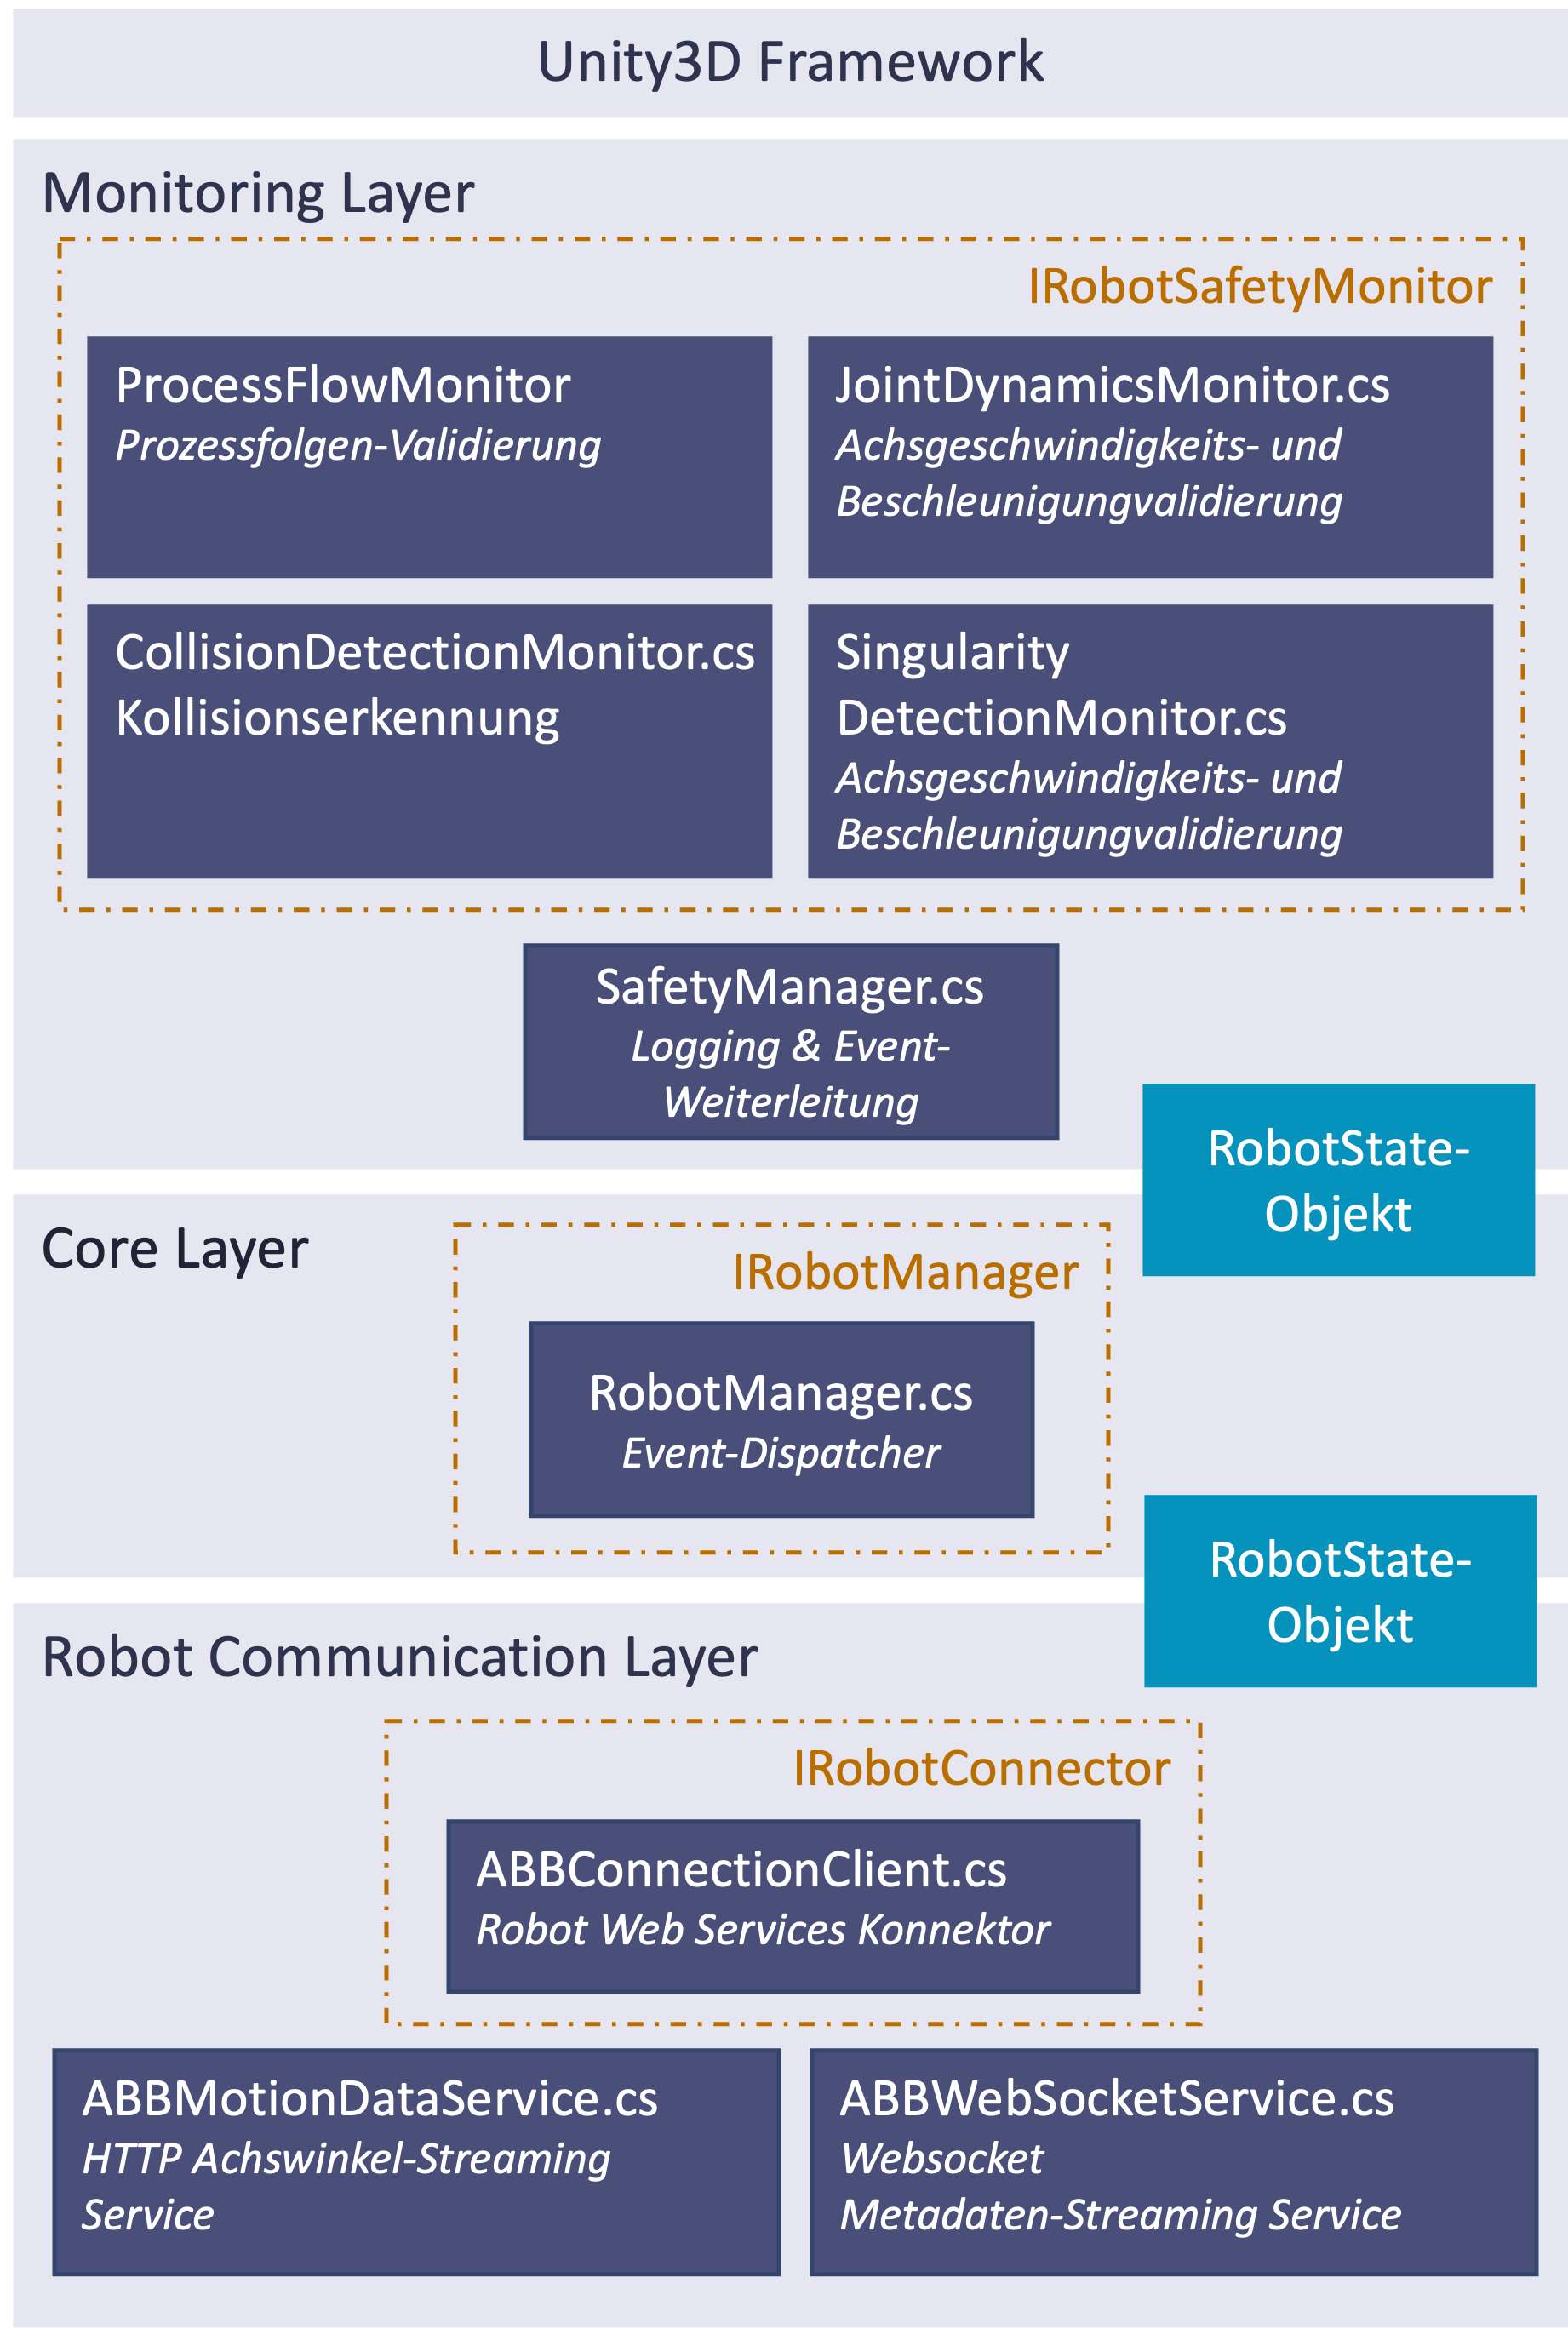
\includegraphics[width=10cm]{Figures/LayerArchitekturFramework.png}
	\caption{Schichtenarchitektur des Frameworks mit den wichtigsten zugehörigen
		Modulen. Module mit grüner Umrandung werden durch ine Interface formalisiert.}
	\label{figure:layer}
\end{figure}

\dirtree{%
	.1 RobotSystem/.
	.2 Core/.
	.3 RobotManager.cs.
	.3 RobotState.cs.
	.3 RobotSafetyManager.cs.
	.3 SafetyEvent.cs.
	.3 RobotStateSnapshot.cs.
	.3 Part.cs.
	.3 Station.cs.
	.3 RapidTargetGenerator.cs.
	.2 Interfaces/.
	.3 IRobotConnector.cs.
	.3 IRobotDataParser.cs.
	.3 IRobotSafetyMonitor.cs.
	.3 IRobotVisualization.cs.
	.2 ABB/.
	.3 RWS/.
	.4 ABBRWSConnectionClient.cs.
	.4 ABBRWSDataParser.cs.
	.4 ABBMotionDataService.cs.
	.3 ABBFlangeAdapter.cs.
	.2 Monitors/.
	.3 CollisionDetectionMonitor.cs.
	.3 JointDynamicsMonitor.cs.
	.3 ProcessFlowMonitor.cs.
	.3 SingularityDetectionMonitor.cs.
}

\paragraph{Event-Driven Architecture}
Das System nutzt ein durchgängiges Event-System für lose Kopplung:
\begin{itemize}
	\item \texttt{OnRobotStateUpdated}: Zustandsänderungen
	\item \texttt{OnConnectionStateChanged}: Verbindungsstatus
	\item \texttt{OnSafetyEventDetected}: Sicherheitsereignisse
	\item \texttt{OnMotorStateChanged}: Motorstatusänderungen
\end{itemize}

\paragraph{SafetyEvent und RobotStateSnapshot}
Das \texttt{SafetyEvent}-System implementiert ein umfassendes Ereignismodell:
\begin{itemize}
	\item \textbf{SafetyEvent}: Unveränderliches Value Object für Sicherheitsereignisse
	\item \textbf{RobotStateSnapshot}: Immutable Zustandserfassung zum Ereigniszeitpunkt
	\item \textbf{Ereignistypen}: Info, Warning, Critical mit konfigurierbaren Schwellwerten
	\item \textbf{Kontextdaten}: Vollständige Roboterzustandserfassung für Forensik
\end{itemize}

\paragraph{Datenformate}
\begin{itemize}
	\item \textbf{HTTPS/HTTP}: RESTful API-Zugriff mit Digest-Authentifizierung
	\item \textbf{WebSocket Secure (WSS)}: Bidirektionale Echtzeit-Kommunikation
	\item \textbf{XML}: Strukturierte Datenübertragung mit Schema-Validierung
	\item \textbf{JSON}: Interne Datenrepräsentation und Logging-Format
\end{itemize}

\section{Implementierung der Module}

\subsection{Allgemeine Struktur}

\subsection{Prozessfolgen}
\label{ssec:Prozessfolgen}
% Überprüfung der korrekten Abfolge von Aktionen...
User Input: Simulationsumgebung und Verbindung zu Robot Studio

Wie kann ich Prozessfolgen überprüfen? Prozessfolge: Folge and Arbeitsschritten
eines Arbeitsprozesses, hier Roboter -> Was wird in welcher Reihenfolge wohin
bewegt? Wie kann ich das Messen? - Bewegt sich das Werkstück von Position Start
zu Position Ziel? - Bewegen sich die Werkstücke in der richtigen Reihenfolge
von Start zu Ziel? Benötigt: Definition von Start \& Zielpositionen einzelner
Werkstücke

\subsection{Kollisionen}
\subsubsection{Theoretische Grundlagen}

Kollisionen eines Roboters mit Objekten im Arbeitsraum stellen eine zentrales
Problem beim Neuentwurf und der Testung neu entwickelten Codes dar. Kollidiert
ein industrieller Roboter unvorhergesehen mit seinem Arbeitsraum, kann dies im
schlimmsten Fall zu einem Ausfall des am Produktionsschrit beteiligen Roboters
\subsubsection{Implementierung}



\subsection{Singularity Detection Monitor} \label{ssec:Singularitaeten}
Im Folgenden wird der Singularity Detection Monitor zur Erkennung von
singulären Gelenkpositionen des Roboters näher erläutert. Ziel ist es,
Handgelenks-, Ellbogen- und Schulter-Singularitäten festzustellen und beim
Auftreten Events mit relevanten Informationen wie Achswinkeln, Nähe zur
Singularität sowie verbleibende Manipulierbarkeit des Roboters auszugeben.

\subsubsection{Theoretische Grundlagen der Singularitätsdetektion}
\label{sssec:Theorie_Singularitaeten}
Kinematische Singularitäten stellen ein fundamentales Problem in der
Robotersteuerung dar und treten auf, wenn die Jacobi-Matrix des Roboters ihren
vollen Rang verliert. In diesen Konfigurationen verliert der Roboter die
Fähigkeit, sich in bestimmte Richtungen im kartesischen Raum zu bewegen, was zu
Kontrollverlust und potentiell gefährlichen Situationen führen
kann.\vglcite{siciliano2016robotics}

Eine kinematische Singularität tritt auf,
wenn die Jacobi-Matrix $\mathbf{J}(\boldsymbol{\theta})$, welche des Roboters
ihren vollen Rang verliert:
\begin{equation}
  \text{rank}(\mathbf{J}(\boldsymbol{\theta})) < \min(m, n)
  \label{eq:singularity_condition}
\end{equation} wobei
$\mathbf{J}(\boldsymbol{\theta}) \in \mathbb{R}^{m \times n}$ die Jacobi-Matrix,
$\boldsymbol{\theta}$ der Gelenkwinkelvektor, $m$ die Anzahl der Freiheitsgrade
im kartesischen Raum und $n$ die Anzahl der Robotergelenke darstellt.

Die Jacobi-Matrix beschreibt die Beziehung zwischen Gelenkgeschwindigkeiten
$\dot{\boldsymbol{\theta}}$ und kartesischen Geschwindigkeiten des TCP
$\mathbf{v}$:
\begin{equation} \mathbf{v} = \mathbf{J}(\boldsymbol{\theta})
  \dot{\boldsymbol{\theta}} \label{eq:jacobian_velocity}
\end{equation}

Tritt eine Singularität auf, so wird die Jacobi-Matrix singulär:
\begin{equation} \det(\mathbf{J}) = 0 \label{eq:jacobian_singularity}
\end{equation} Dadurch wird die inverse Kinematik nicht
eindeutig lösbar ist und es können theoretisch unendliche
Gelenkgeschwindigkeiten auftreten.\vglcite{nakamura1991advanced}

\subsubsection{Frameworkspezifisches Vorgehen}
Im Rahmen der praktischen Implementierung wird hier ein auf Schwellwerten und
absoluten sowie winkelbasierten Entfernungen zur Singularität angewendet. Durch
die Anwendung der rein mathematischen Definition ließe sich zwar jede beliebige
Singularität in einer seriellen Kinematik erkennen, jedoch bleiben die
betroffenen Gelenke und Art der Singularität ungewiss und müssten iterativ
bestimmt werden. Daher wird hier eine pragmatische Berechnungsmethodik
verwendet.

Für serielle Robotermanipulatoren mit sechs Freiheitsgraden, wie den hier
verwendeten ABB IRB 6700, können drei primäre Singularitätstypen unterschieden
werden: Schultersingularitäten, Ellbogensingularitäten und
Handgelenksingularitäten.\vglcite{spong2006robot}

\paragraph{Schultersingularitäten} treten auf, wenn sich das
Handgelenkszentrum (Schnittpunkt der Achsen 4, 5, 6) direkt über oder nahe der
Rotationsachse des ersten Gelenks befindet:

\begin{equation}
  \sqrt{x_{wc}^2 + y_{wc}^2} < \epsilon
  \label{eq:shoulder_singularity}
\end{equation}

wobei $(x_{wc}, y_{wc})$ die Position des Handgelenkszentrums in der XY-Ebene
und $\epsilon$ der Singularitätsschwellenwert ist.

\paragraph{Ellbogensingularitäten} treten auf, wenn der Roboter die
Grenzen seines
Arbeitsraums erreicht. Dies geschieht typischerweise bei vollständig
ausgestreckter oder eingeklappter Konfiguration. Beim
Knickarmrobotern wie dem IRB 6700
verläuft die Rotationsachse des vierten Gelenks nicht direkt durch
den Ursprung vom
dritten Gelenk, sondern ist durch eine Translation verschoben. Das impliziert,
dass die vollständige Streckung des Armes nicht durch einen Winkel
von $0^\circ$ bzw.
$180^\circ$ auftritt. Hier lässt sich allgemeiner der Zusammenhang der Vektoren
zwischen Gelenk 2 und 3 sowie 2 und 5 anwenden:

\begin{equation}
  \theta = \angle(\vec{v}_{23}, \vec{v}_{25}) \approx 0^\circ \text{
  oder } \theta \approx 180^\circ
  \label{eq:elbow_singularity}
\end{equation}

wobei:
\begin{align}
  \vec{v}_{23} & = \vec{p}_3 - \vec{p}_2 \\
  \vec{v}_{25} & = \vec{p}_5 - \vec{p}_2
\end{align}

mit $\vec{p}_i$ als Position des Gelenks $i$. Die Singularitätsbedingung lautet:
\begin{equation}
  \theta < \epsilon \quad \text{oder} \quad \theta > 180^\circ - \epsilon
\end{equation}

\paragraph{Handgelenksingularitäten} treten auf, wenn die Rotationsachsen der
letzten drei Gelenke (Gelenke 4, 5, 6) kollinear werden. Dies tritt
typischerweise auf, wenn $\theta_5 = 0^\circ$ oder $\theta_5 =
180^\circ$. Mathematisch
beschrieben durch:

\begin{equation}
  \mathbf{z}_4 \parallel \mathbf{z}_6 \text{ oder } |\mathbf{z}_4
  \cdot \mathbf{z}_6| \approx 1
  \label{eq:wrist_singularity}
\end{equation}

wobei $\mathbf{z}_i$ die Rotationsachse (Z-Achse) des $i$-ten Gelenks im
Weltkoordinatensystem darstellt. Beispielhaft ist das Auftreten einer
Handgelenkssingularität in Abbildung~\ref{figure:wristSingularity}
in Unity3D.

\subsubsection{Manipulierbarkeitsindex (Yoshikawa-Maß)} Der von Yoshikawa
\cite{yoshikawa1985manipulability} eingeführte Manipulierbarkeitsindex ist eine
der am häufigsten verwendeten Metriken:
\begin{equation}
  \mu(\boldsymbol{\theta}) =
  \sqrt{\det(\mathbf{J}(\boldsymbol{\theta})\mathbf{J}^T(\boldsymbol{\theta}))}
  \label{eq:yoshikawa_measure}
\end{equation}

Für quadratische Jacobi-Matrizen vereinfacht sich dies zu:
\begin{equation}
  \mu(\boldsymbol{\theta}) = |\det(\mathbf{J}(\boldsymbol{\theta}))|
  \label{eq:yoshikawa_simplified}
\end{equation}

Der Index nimmt Werte zwischen 0 (Singularität) und einem maximalen Wert an,
wobei höhere Werte bessere Manipulierbarkeit indizieren. Die Robotik-Literatur
bietet verschiedene Ansätze zur Behandlung von Singularitäten, die sich in
präventive und reaktive Strategien unterteilen lassen. Um diese in der Praxis
anzuwenden, müssen jedoch teilweise numerische Auswertungen durchgeführt werden,
um Schwellwerte zu erfassen. Daher kommen diese hier nicht zum Einsatz.

Zur zusätzlichen Charakterisierung wird jedoch die Yoshikawa-Manipulierbarkeit
berechnet, da der Wert als Kennzahl für die Nähe zu einer Singularität verwendet
werden kann. Er wird in den Ergebnissen in Kapitel
\ref{sec:singularityauswertung} aufgeführt.

\begin{figure}[H]
  \centering
  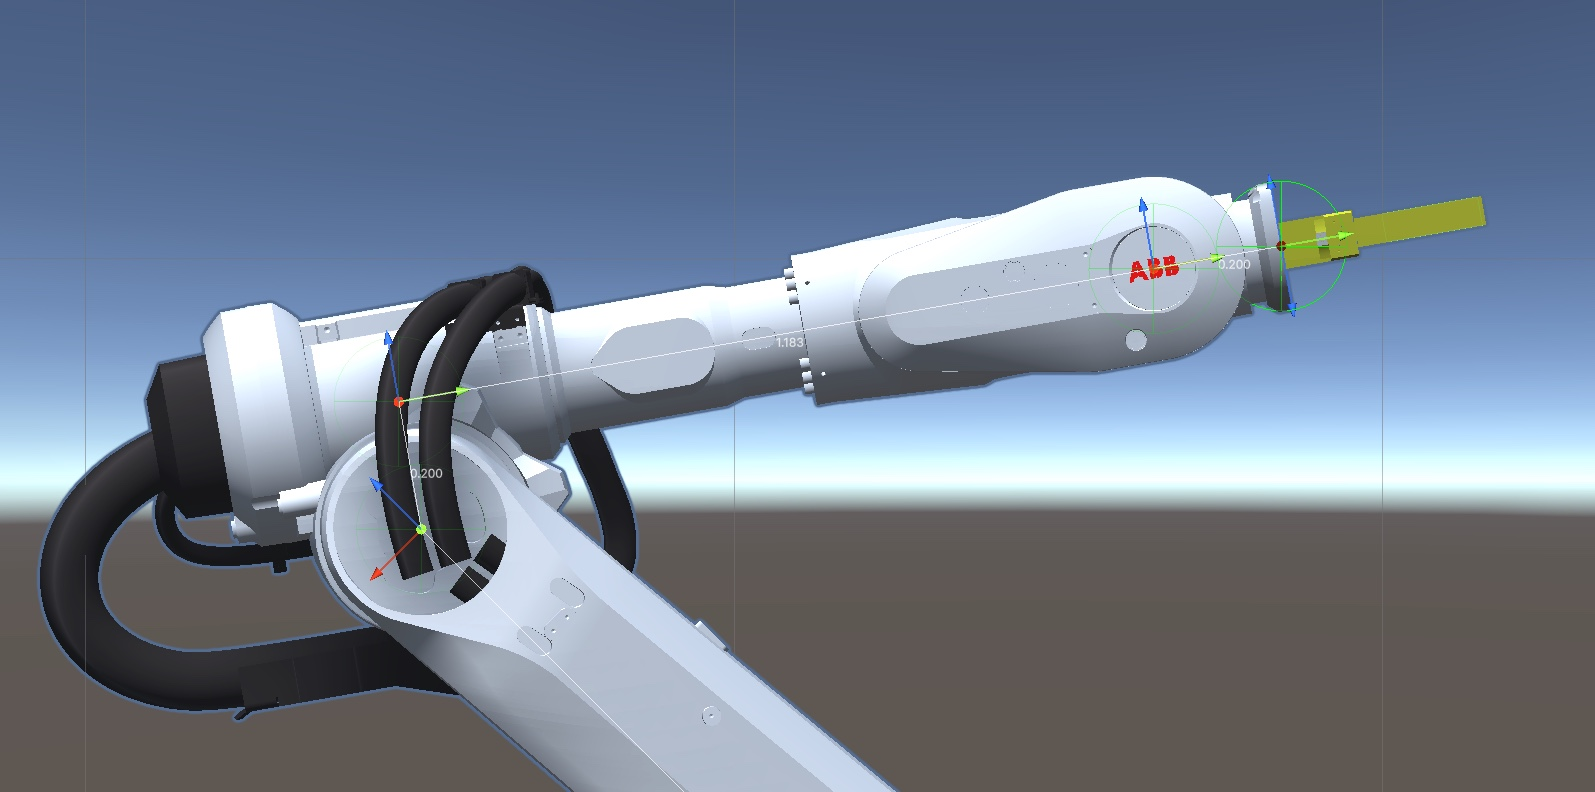
\includegraphics[width=\linewidth]{Figures/wristSingularityScreenshot.jpg}
  \caption{Screenshot einer Handgelenksingularität in Unity mit farbig
  dargestellten Koordinatensystemen der Denavit-Hartenberg-Transformationen }
  \label{figure:wristSingularity}
\end{figure}

\subsubsection{Praktisches Vorgehen}
Nachfolgend werden die Schritte 1 bis 4 zur Prüfung des Vorliegens
einer Singularität dargestellt.

\paragraph{Schritt 1: Positionsberechnung und Achsentransformation}~\\
Die Positionen der relevanten Gelenke werden durch die Anwendung der
Vorwärtstransformation nach Denavit-Hartenberg (DH)
berechnet\vglcite{denavit1955}:
\begin{equation}
  \vec{p}_i = \text{DH}(\theta_1, \ldots, \theta_i) \quad \text{für }
  i = 2, 3, 5
  \label{eq:position_calculation}
\end{equation}

Die Rotationsachsen werden aus den Transformationsmatrizen extrahiert:
\begin{equation}
  \mathbf{z}_i = \mathbf{T}_i[:3, 2] \quad \text{für } i = 1, 4, 6
  \label{eq:axis_extraction}
\end{equation}

\paragraph{Schritt 2: Singularitätsanalyse}~\\
Für jeden Singularitätstyp wird die entsprechende Bedingung überprüft:
\begin{itemize}
  \item \textbf{Schultersingularität:}
    \begin{equation}
      d_{wc} = \sqrt{x_{wc}^2 + y_{wc}^2}
    \end{equation}
    wobei $(x_{wc}, y_{wc})$ die Position des Handgelenkszentrums in
    der XY-Ebene ist.

  \item \textbf{Ellbogensingularität:}
    \begin{equation}
      \theta_{elbow} = \angle(\vec{p}_3 - \vec{p}_2, \vec{p}_5 - \vec{p}_2)
    \end{equation}

  \item \textbf{Handgelenksingularität:}
    \begin{equation}
      c_{46} = |\mathbf{z}_4 \cdot \mathbf{z}_6|
    \end{equation}
\end{itemize}

\paragraph{Schritt 3: Schwellwertvergleich}~\\
\begin{table}[H]
  \centering
  \begin{tabular}{l l l}
    \hline
    \textbf{Singularitätstyp} & \textbf{Beispiel-Schwellwert}      &
    \textbf{Bedingung}                            \\
    \hline
    Schulter                  & $\tau_{\text{shoulder}} = 100$ mm  &
    $d_{wc} < \tau_{\text{shoulder}}$             \\
    Ellbogen                  & $\tau_{\text{elbow}} = 5^{^\circ}$ &
    $\theta_{elbow} < \tau_{\text{elbow}}$ oder   \\
    &                                    & $\theta_{elbow} >
    180^\circ - \tau_{\text{elbow}}$ \\
    Handgelenk                & $\tau_{\text{wrist}} = 5^{^\circ}$ &
    $c_{46} > \tau_{\text{wrist}}$                \\
    \hline
  \end{tabular}
  \caption{Singularitätsschwellwerte und Detektionsbedingungen}
  \label{tab:singularity_thresholds}
\end{table}

\paragraph{Schritt 4: Manipulierbarkeitsberechnung}~\\
Für detektierte Singularitäten wird ein approximierter Manipulierbarkeitsindex
nach Yoshikawa berechnet:

\begin{equation}
  w = \sqrt{\det(\mathbf{J}(\theta)\mathbf{J}^T(\theta))}
  \label{eq:manipulability}
\end{equation}

Ein kleiner Wert von $w$ indiziert die Nähe zu einer singulären Konfiguration.
Das entwickelte Framework implementiert eine winkelbasierte
Singularitätsdetektion, die geometrische Eigenschaften der Roboterkinematik
direkt nutzt, anstatt auf rechenintensive Jacobi-Matrix-Berechnungen angewiesen
zu sein. Die achsenbasierte Methode basiert auf der Erkenntnis, dass
Handgelenks- und Ellbogensingularitäten geometrisch durch die
Kollinearität von Rotationsachsen
charakterisiert werden können. Schultersingularitäten werden analog durch die
Entfernung des ersten Gelenks zum Handgelenkzentrum in der XY-Ebene
festgestellt.

\subsubsection{Konkrete Implementierung der Detektionsmethoden}
\label{sssec:Implementierung_Detektionsmethoden}
Die Implementierung des \texttt{SingularityDetectionMonitor} nutzt die
Vorwärtskinematik des Preliy Flange Frameworks zur Berechnung der
Gelenkpositionen. Die zentrale Methode \texttt{ComputeJointPosition} berechnet
die kartesische Position eines beliebigen Gelenks durch sukzessive Anwendung
der Denavit-Hartenberg-Transformationsmatrizen (vgl.
Abbildung~\ref{listing:forwardKinematic}).

\begin{figure}[H]
  \inputminted[fontsize=\footnotesize]{csharp}{code-snippets/CalculateJointPos.cs}
  \caption{Vorwärtskinematik zur Positionsberechnung}
  \label{listing:forwardKinematic}
\end{figure}

Die Methode \texttt{ComputeJointPosition} in Abbildung
\ref{listing:forwardKinematic} implementiert die klassische
Vorwärtskinematik durch
Multiplikation homogener Transformationsmatrizen. Jede Matrix $\mathbf{T}_i$
wird aus den DH-Parametern $(\alpha_i, a_i, d_i, \theta_i)$ konstruiert, wobei
$\theta_i$ der aktuelle Gelenkwinkel plus einem konstanten Offset ist. Die
resultierende Transformationsmatrix beschreibt die Position und Orientierung des
Gelenks im Basiskoordinatensystem.\\

Das Framework nutzt Unitys \texttt{Matrix4x4}-Klasse für die
Transformationsberechnungen und die \texttt{GetPosition()}-Methode zur
Extraktion der Translationskomponente. Die Koordinatentransformation zwischen
dem DH-Parametersystem und Unitys linkshändigem Y-up Koordinatensystem wird
dabei durch die Methode \texttt{HomogeneousMatrix.CreateRaw()} des
Flange-Frameworks transparent gehandhabt. Das ermöglicht eine nahtlose
Integration der mathematischen Robotik-Konzepte in die Unity-Umgebung, während
die Echtzeitfähigkeit durch eventgetriebene Berechnung gewährleistet ist.
Bei der Detektion einer Singularität bzw. dem Unterschreiten des im Unity-Editor
definierten Grenzwertes wird ein \texttt{SafetyEvent}-Objekt
instanziert und an die
\texttt{SafetyMonitor} Klasse weitergegeben. Darin werden zusätzlich
Event-Metadaten zu den
Daten der Gelenkwinkelabstände ausgegeben. Sobald der
kritische Bereich verlassen wurde, wird ein weiteres
\texttt{SafetyEvent} ausgegeben, um
den Bereich, in welcher die Singularität auftritt, abstecken zu können.


\section{Testumgebung und -setup}
\subsection{Aufbau der Roboterzelle}
\subsection{Implementierung in Unity}
\section{Datenaufzeichung und Logging}
\subsection{JSON-Struktur}
\subsection{Speicherung}
